\section{Messger\"{a}te}
Bei der Konzeption der Versuchsaufbauten sollte anfangs darauf geachtet werden, dass mit diesen verschiedene Messger\"{a}te unterschiedlicher Hersteller getestet werden k\"{o}nnen. Im Verlauf des Projekts wurde zur Vereinfachung des Konzeptentwurfs nach Absprache mit dem Auftraggeber sich darauf geeinigt, sich auf die Messger\"{a}te \textbf{Fast Mobility Particle Sizer Spectrometer Model 3091} (kurz FMPS 3091) und \textbf{Optical Particle Sizer Model 3330} (kurz OPS 3330) der Firma \textbf{TSI} zu konzentrieren. 
\\
Es bestand dennoch weiterhin die Schwierigkeit geeignete Anforderungen zu identifizieren, die die Versuchsaufbauten erf\"{u}llen m\"{u}ssen, um sie zumindest auf die Ger\"{a}te FMPS 3091 und OPS 3330 anwenden zu k\"{o}nnen. Die Gr\"{u}nde hierf\"{u}r liegen in ihren unterschiedlichen Leistungen und Funktionsrinzipien. Abbildung \ref{fig:verfahren} zeigt einen \"{U}berblick \"{u}ber die heutigen verf\"{u}gbaren Messverfahren. Die Wahl eines Verfahrens h\"{a}ngt unter anderem davon ab, welche Partikelgr\"{o}{\ss}en gemssen werden sollen. 
\begin{figure}[H]
	\myfloatalign
	{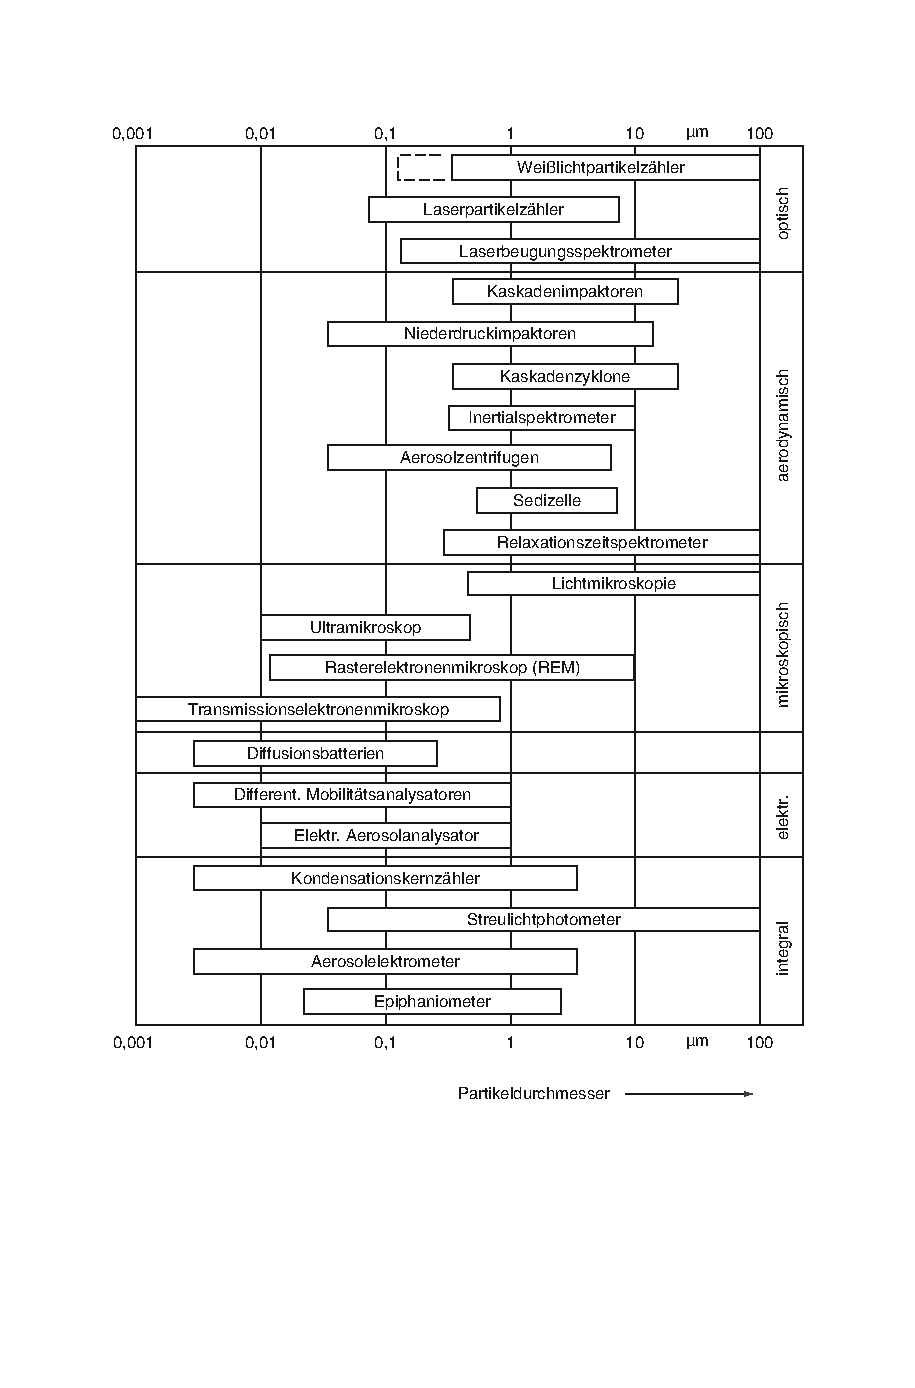
\includegraphics[width=.6\linewidth]{gfx/measuring_dev/partikelmessverfahren.pdf}} \quad
	\caption[\"{U}bersicht \"{u}ber gebr\"{a}uchliche Partikelmessverfahren\cite{reinraum}]
	{\"{U}bersicht \"{u}ber gebr\"{a}uchliche Partikelmessverfahren\cite{reinraum}}
	\label{fig:verfahren}
\end{figure}
\newpage
Optische Partikelz\"{a}hler arbeiten nach dem physikalischen Prinzip, dass beleuchtete Partikel das Licht aus seiner urspr\"{u}nglichen Ausbreitungsrichtung ablenken (Abbildung \ref{fig:optischer_messer}). Bei diesen passiert jeder einzelne Partikel ein Messvolumne, in dem er von Licht bestrahlt wird und dann mit Hilfe eines Detektors die Intensit\"{a}t des gestreuten Lichts und die Anzahl der gestreuten Lichtimpulse gemessen. Die Intensit\"{a}t l\"{a}sst Aufschl\"{u}sse \"{u}ber die Partikelgr\"{o}{\ss}e ziehen, bei einem bekannten Volumenstrom und vordefinierter Messdauer l\"{a}sst sich \"{u}ber die Anzahl der Lichtimpulse die Partikelkonzentration bestimmen. Bei moderneren Ger\"{a}ten wie dem OPS 3330 geschieht die optische Messung mit Hilfe eines Lasers (Abbildung \ref{fig:laser_schwert}). Hierbei kommt zus\"{a}tzlich ein Parabolspiegel hinzu, mit dem das gestreute Licht von einem Detektor gesammelt wird. Bei diesem Messprinzip ist es wichtig, dass jeder Partikel das Messvolumen einzeln durchl\"{a}uft. Falls zwei oder mehr Partikel das Messvolumen gleichzeitig durchlaufen, werden sie als ein Gro{\ss}es gewertet. Dieser Effekt wird als Koinzidenz bezeichnet. Es existieren zwei Methoden, um diesen Effekt zu vermeiden. Die erste Methode arbeitet aerodynamisch, bei welcher der Aerosolstrahl von einem Mantel aus reiner Luft umgeben ist und mittels einer Ansaugd\"{u}se als d\"{u}nner Strahl austritt (Abbildung \ref{fig:aerodynamisch_trennung}).\\
Die zweite Methode arbeitet rein optisch mit Hilfe von zwei Blenden, die den Bereich des zu empfangenden Lichts einschr\"{a}nken (Abbildung \ref{fig:optisch_trennung}).

\begin{figure}[H]
	\myfloatalign
	{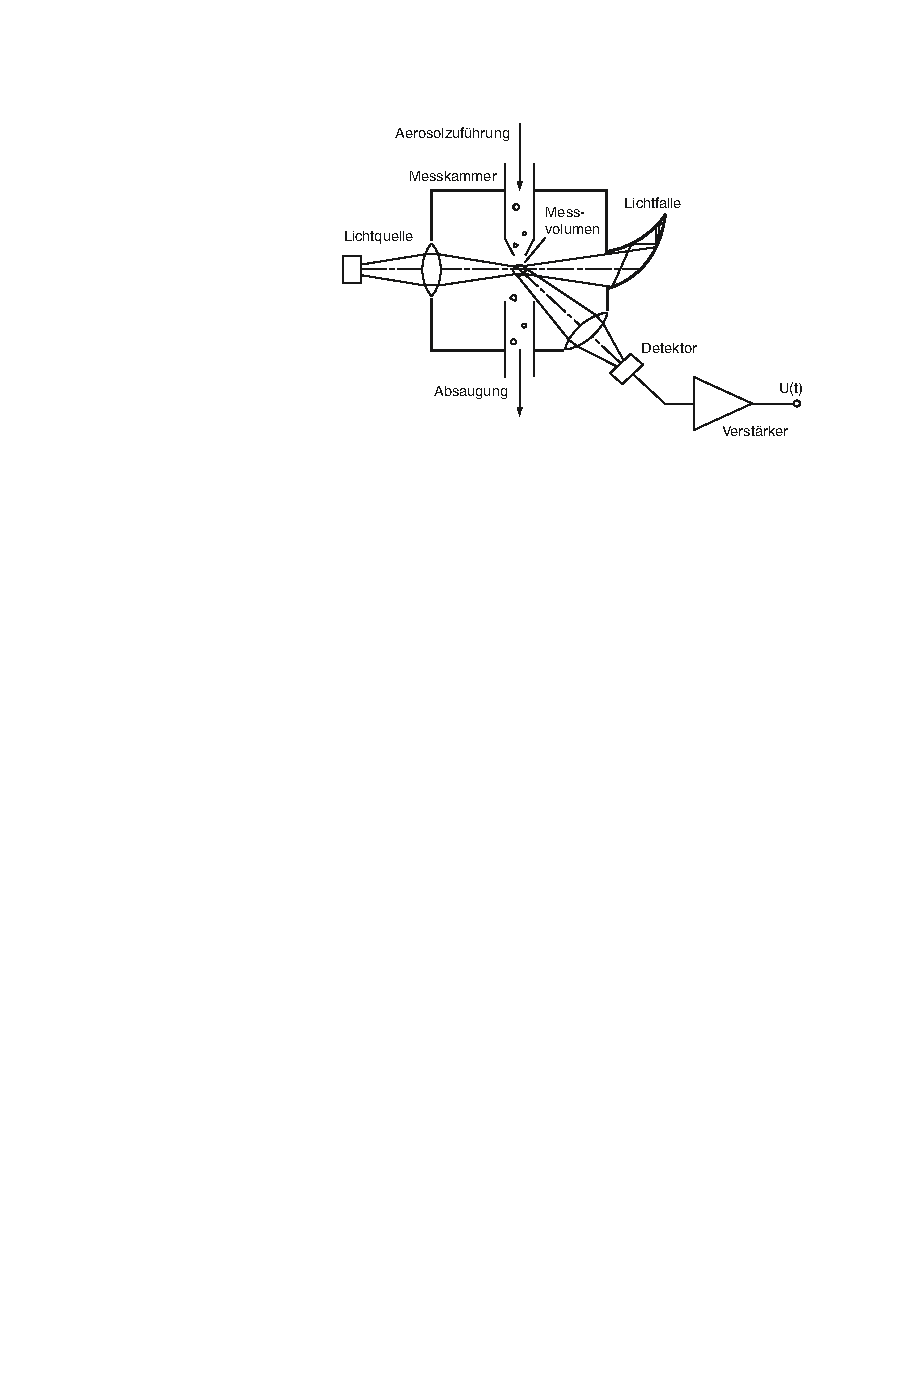
\includegraphics[width=.5\linewidth]{gfx/measuring_dev/optischer_messer.pdf}} \quad
	\caption[Funktionsprinzip eines optischen Partikelz\"{a}hlers (Quelle: \cite{reinraum}, S.75)]
	{Funktionsprinzip eines optischen Partikelz\"{a}hlers\cite{reinraum}}
	\label{fig:optischer_messer}
\end{figure}

\begin{figure}[H]
	\myfloatalign
	\subfloat[Seitenansicht]
	{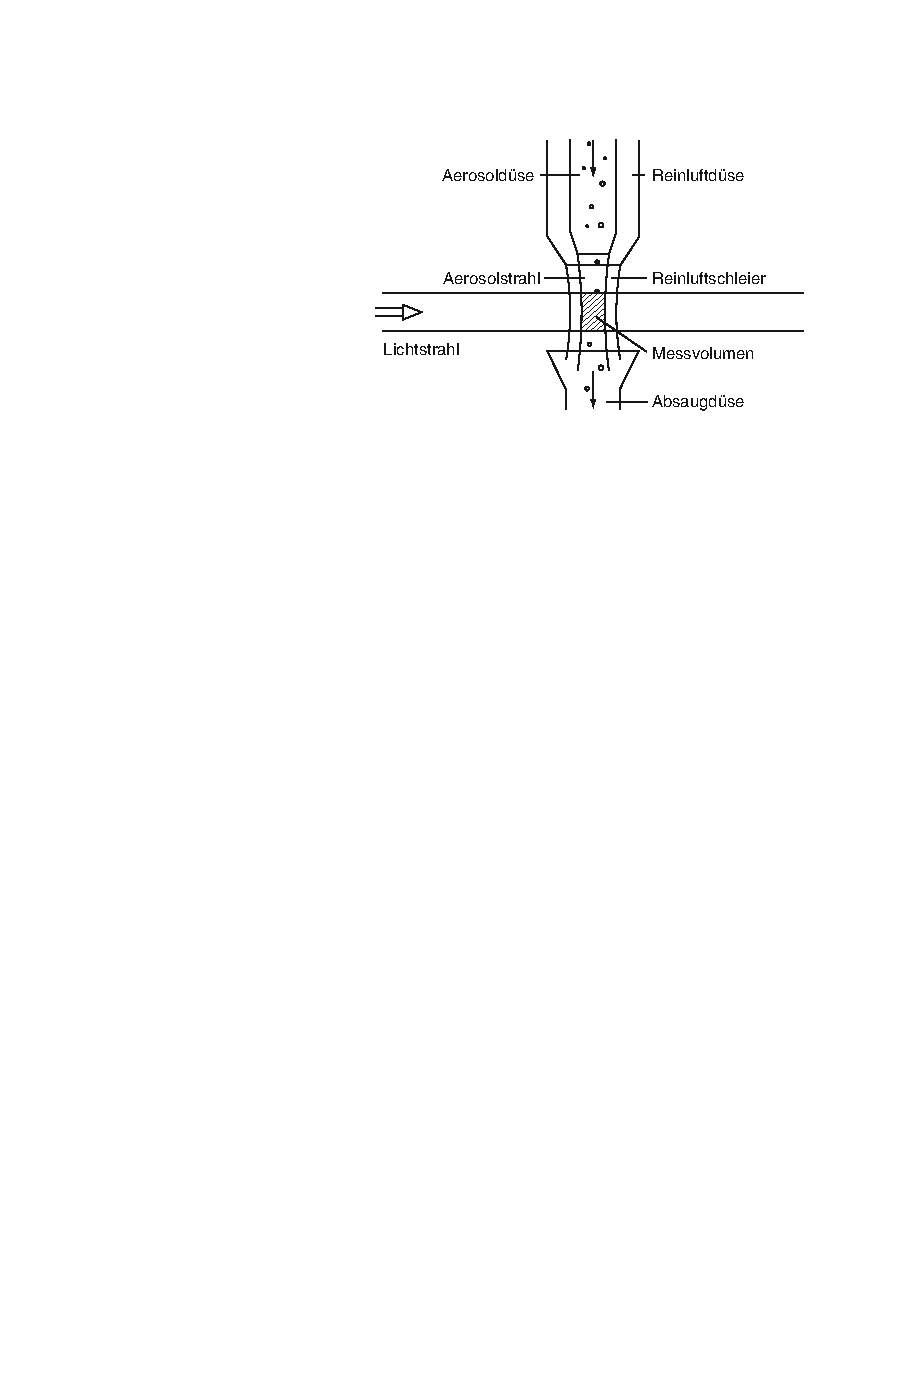
\includegraphics[width=.45\linewidth]{gfx/measuring_dev/aerodynamisch_seite.pdf}} \quad
	\subfloat[Von-Oben Ansicht]
	{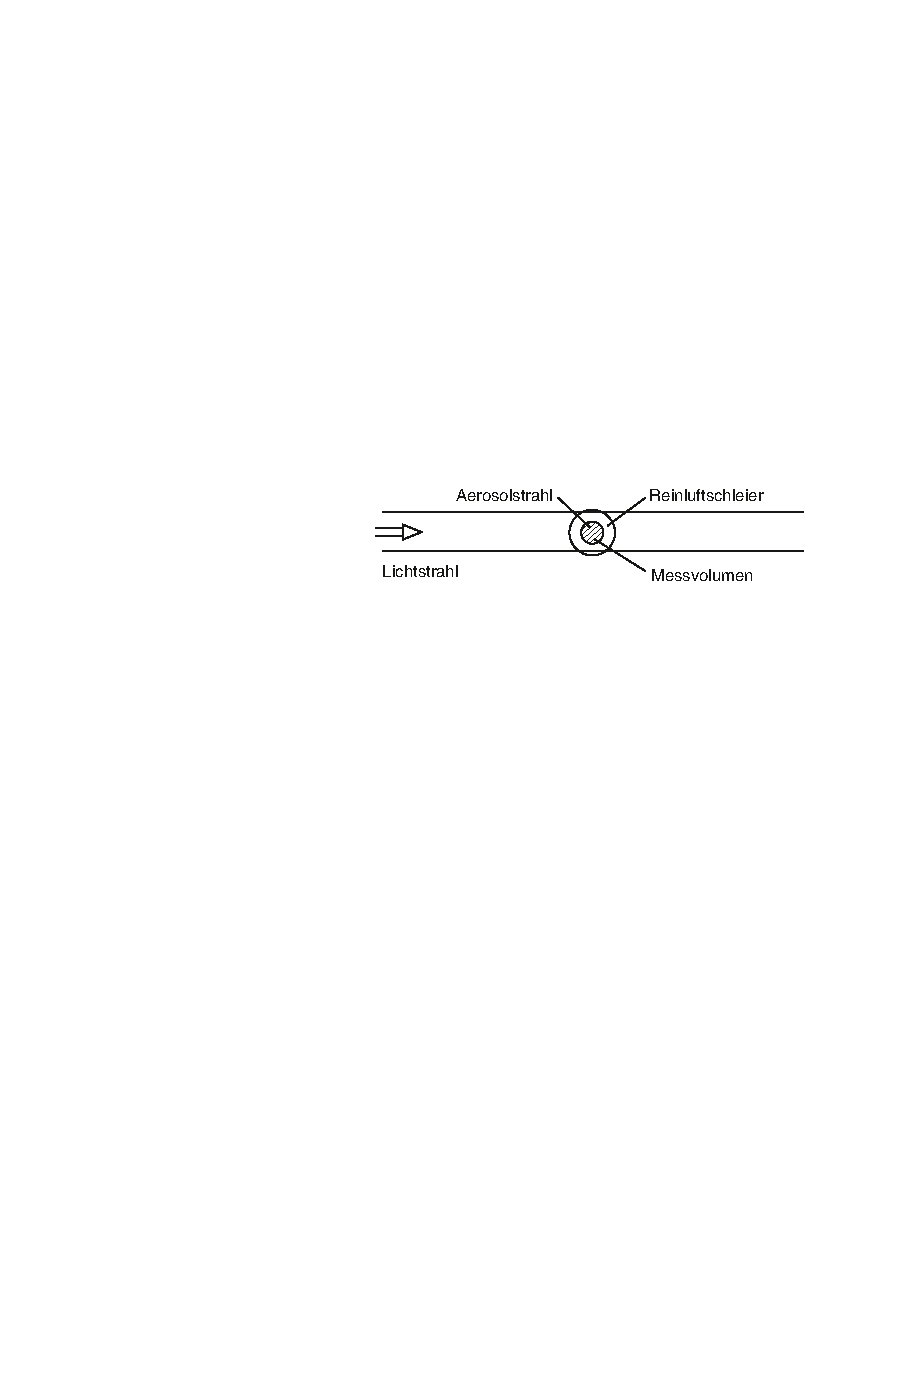
\includegraphics[width=.45\linewidth]{gfx/measuring_dev/aerodynamisch_oben.pdf}}
	\caption[Messvolumentrennung durch aerodynamische Fokussierung\cite{reinraum}]
	{Messvolumentrennung durch aerodynamische Fokussierung\cite{reinraum}}
	\label{fig:aerodynamisch_trennung}
\end{figure}

\begin{figure}[H]
	\myfloatalign
	\subfloat[Seitenansicht]
	{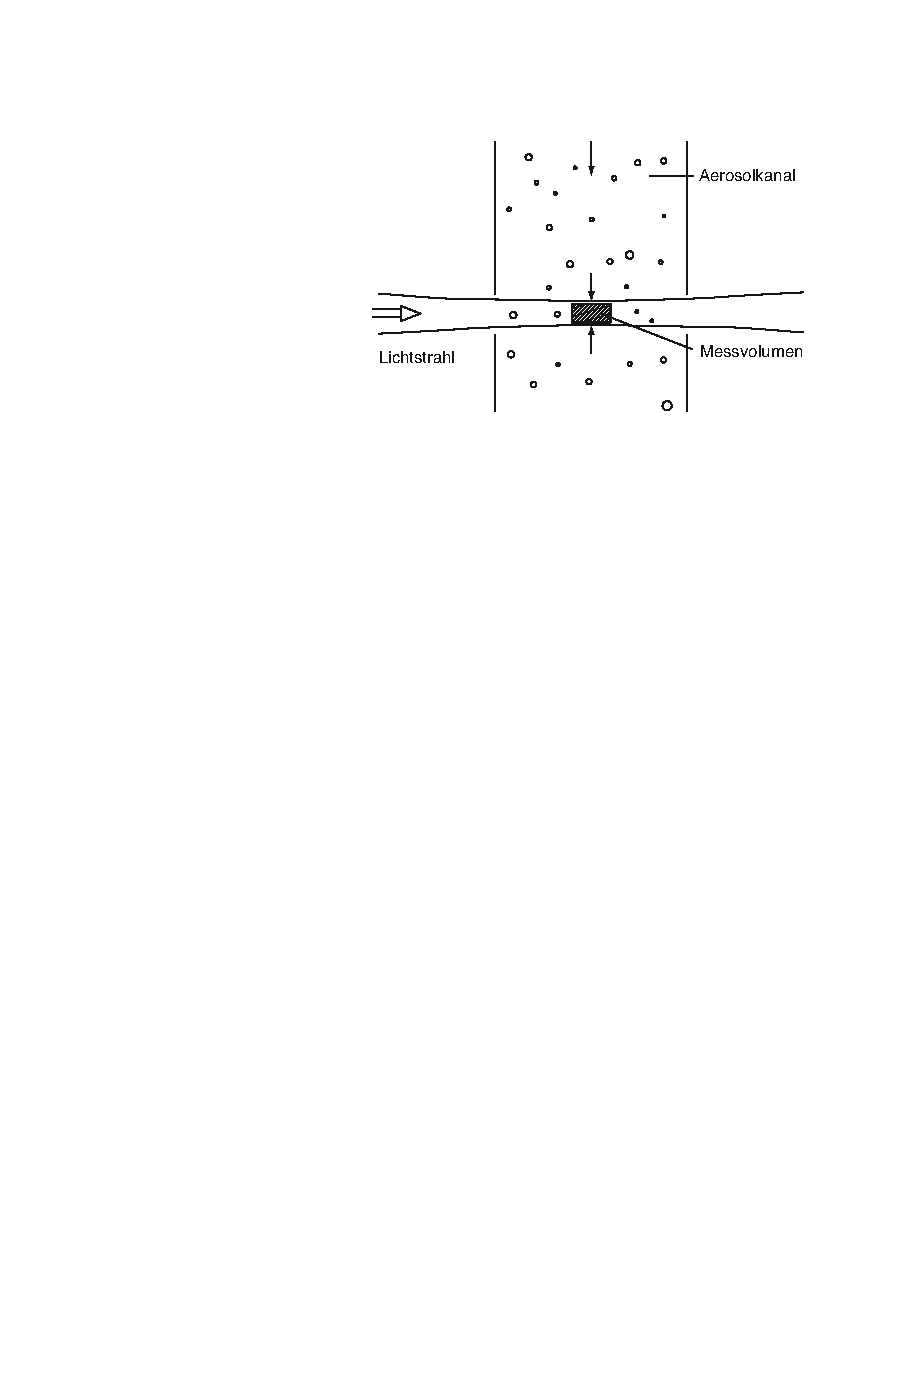
\includegraphics[width=.45\linewidth]{gfx/measuring_dev/optisch_seite.pdf}} \quad
	\subfloat[Von-Oben Ansicht]
	{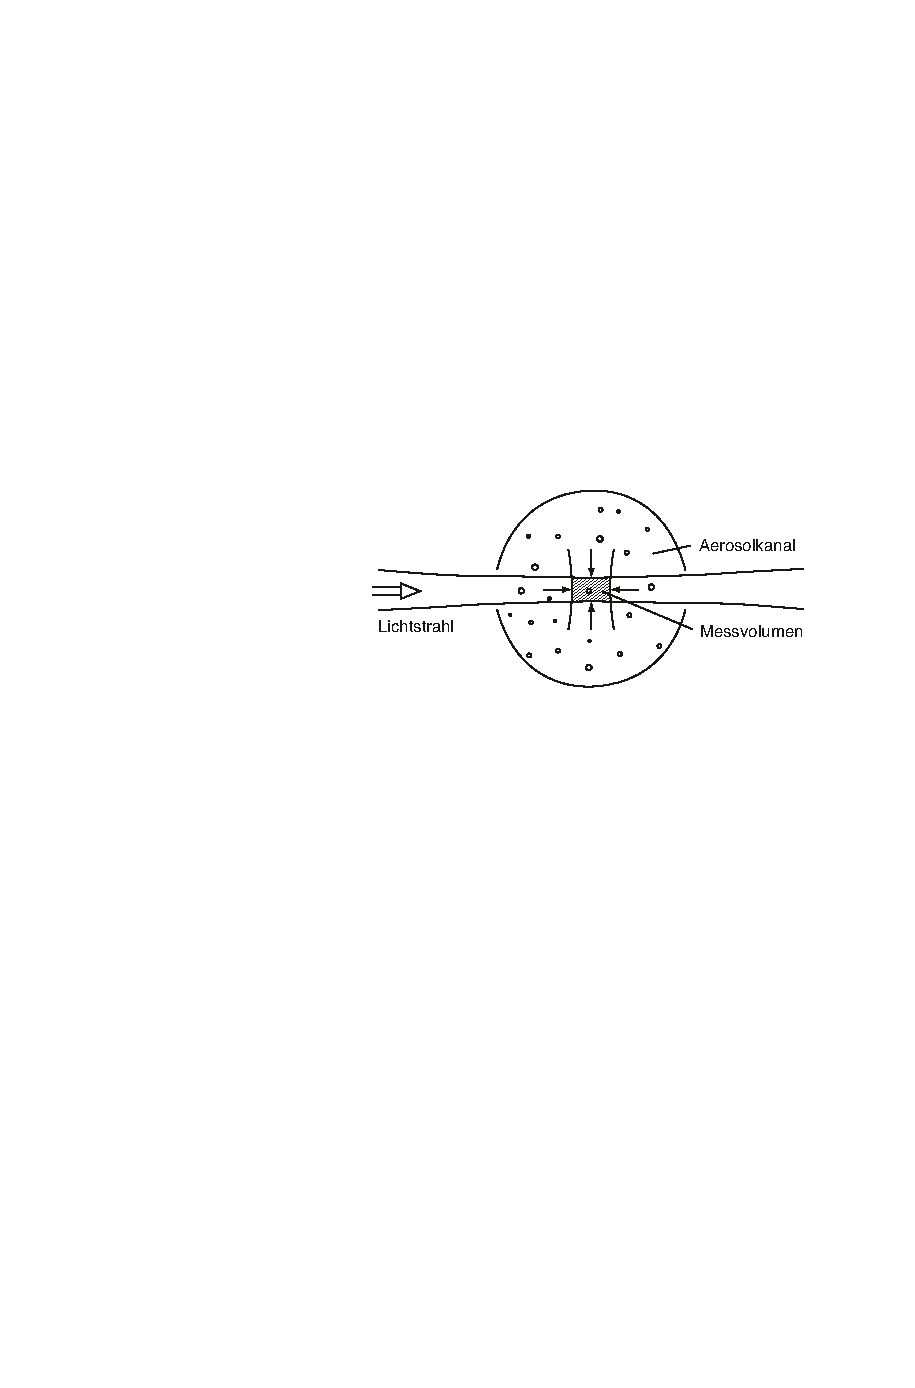
\includegraphics[width=.45\linewidth]{gfx/measuring_dev/optisch_oben.pdf}}
	\caption[Messvolumentrennung mit Hilfe von Blenden\cite{reinraum}]
	{Messvolumentrennung mit Hilfe von Blenden\cite{reinraum}}
	\label{fig:optisch_trennung}
\end{figure}

Elektrische Pertikelz\"{a}hler, wie der FMPS 3091 hingegen ben\"{o}tigen keine speziellen Techniken, um Partikel einzeln zu erfassen. Beim FMPS 3091 werden die Partikel positiv aufgeladen und anschlie{\ss}end mit einem reinen Luftstrom in das Messvolumen gef\"{u}hrt, in welchem sich eine Elektrode befindet und ein elektrisches Feld erzeugt. Elektrometer, welche um die Eletrode angebracht sind und verschieden empfindlich sind, messen die geladenen Partikel (Abbildung \ref{fig:laser_schwert}).

\begin{figure}[H]
	\myfloatalign
	\subfloat[Elektrische Messung beim FMPS 3091\cite{fmps_3091}]
	{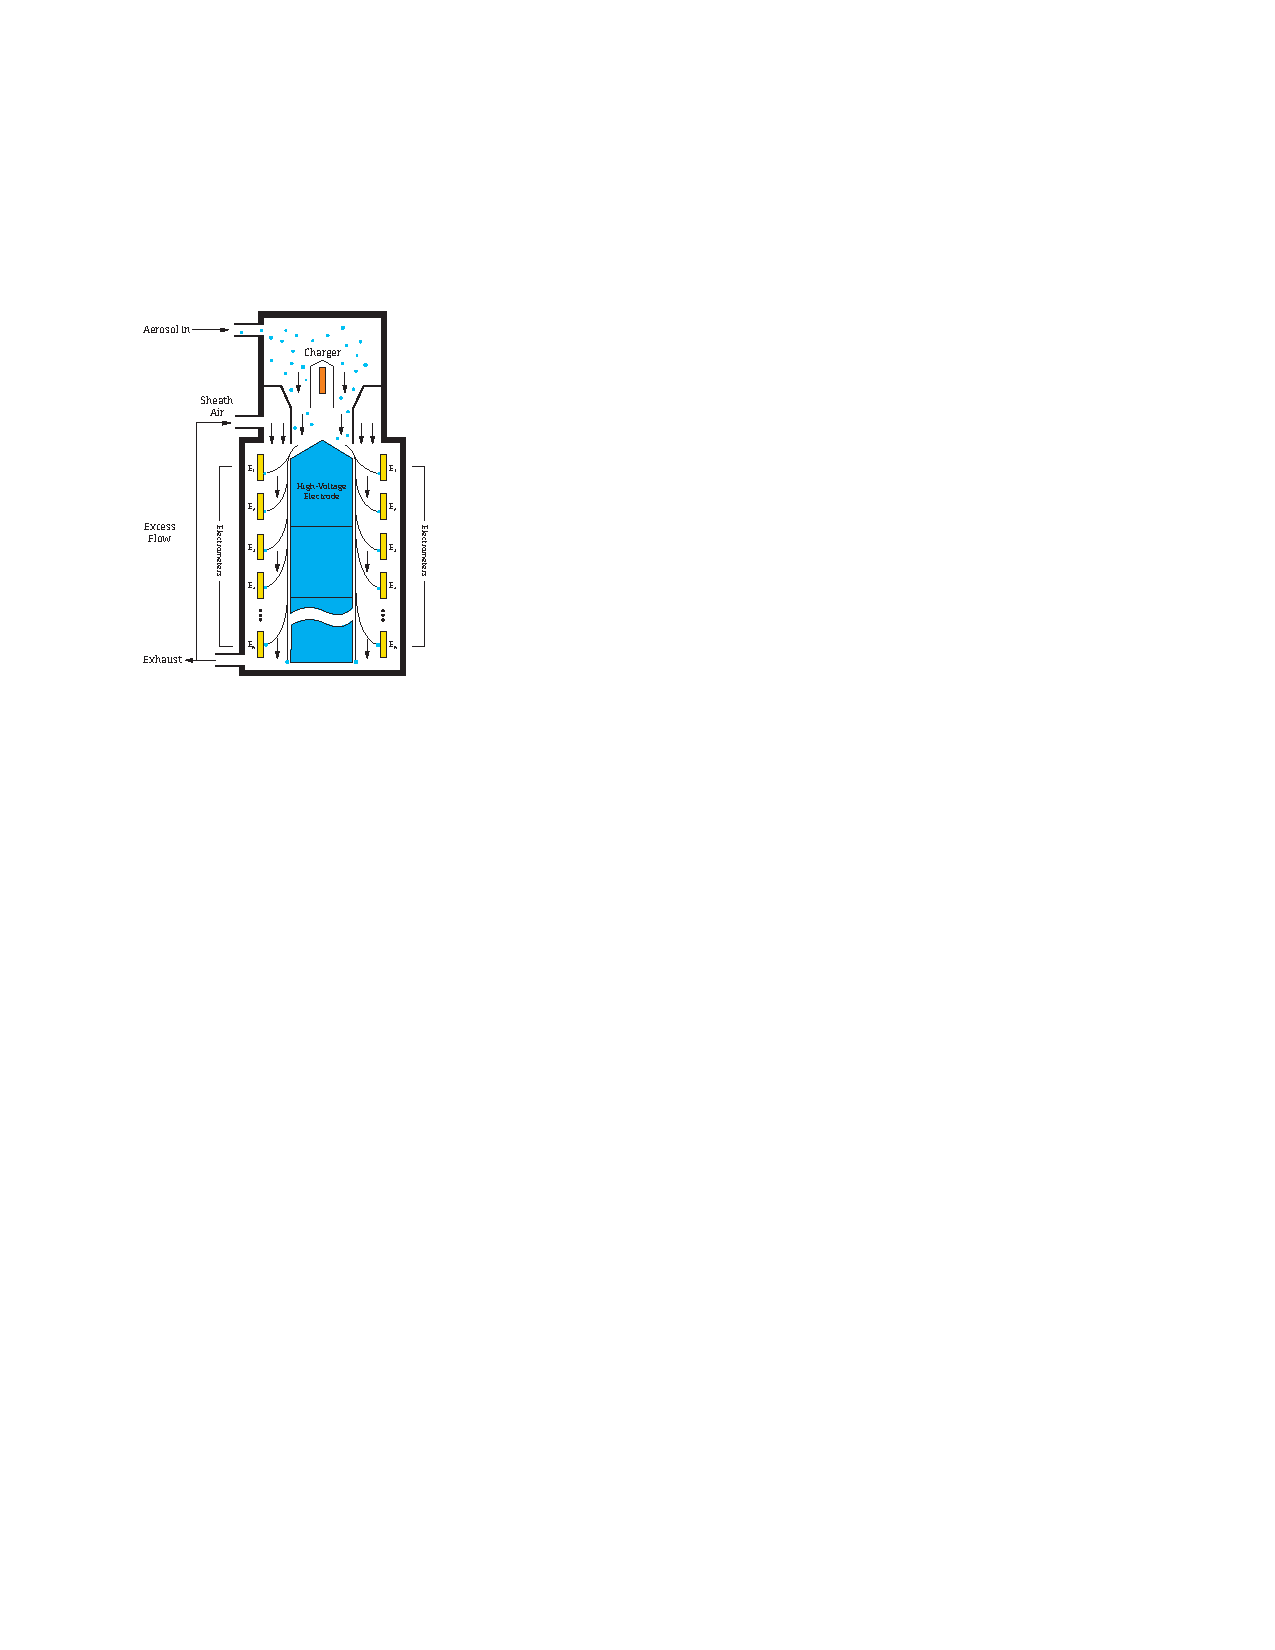
\includegraphics[width=.45\linewidth]{gfx/measuring_dev/fmps_3091.pdf}} \quad
	\subfloat[Lasermessung beim OPS 3330\cite{ops_3330}]
	{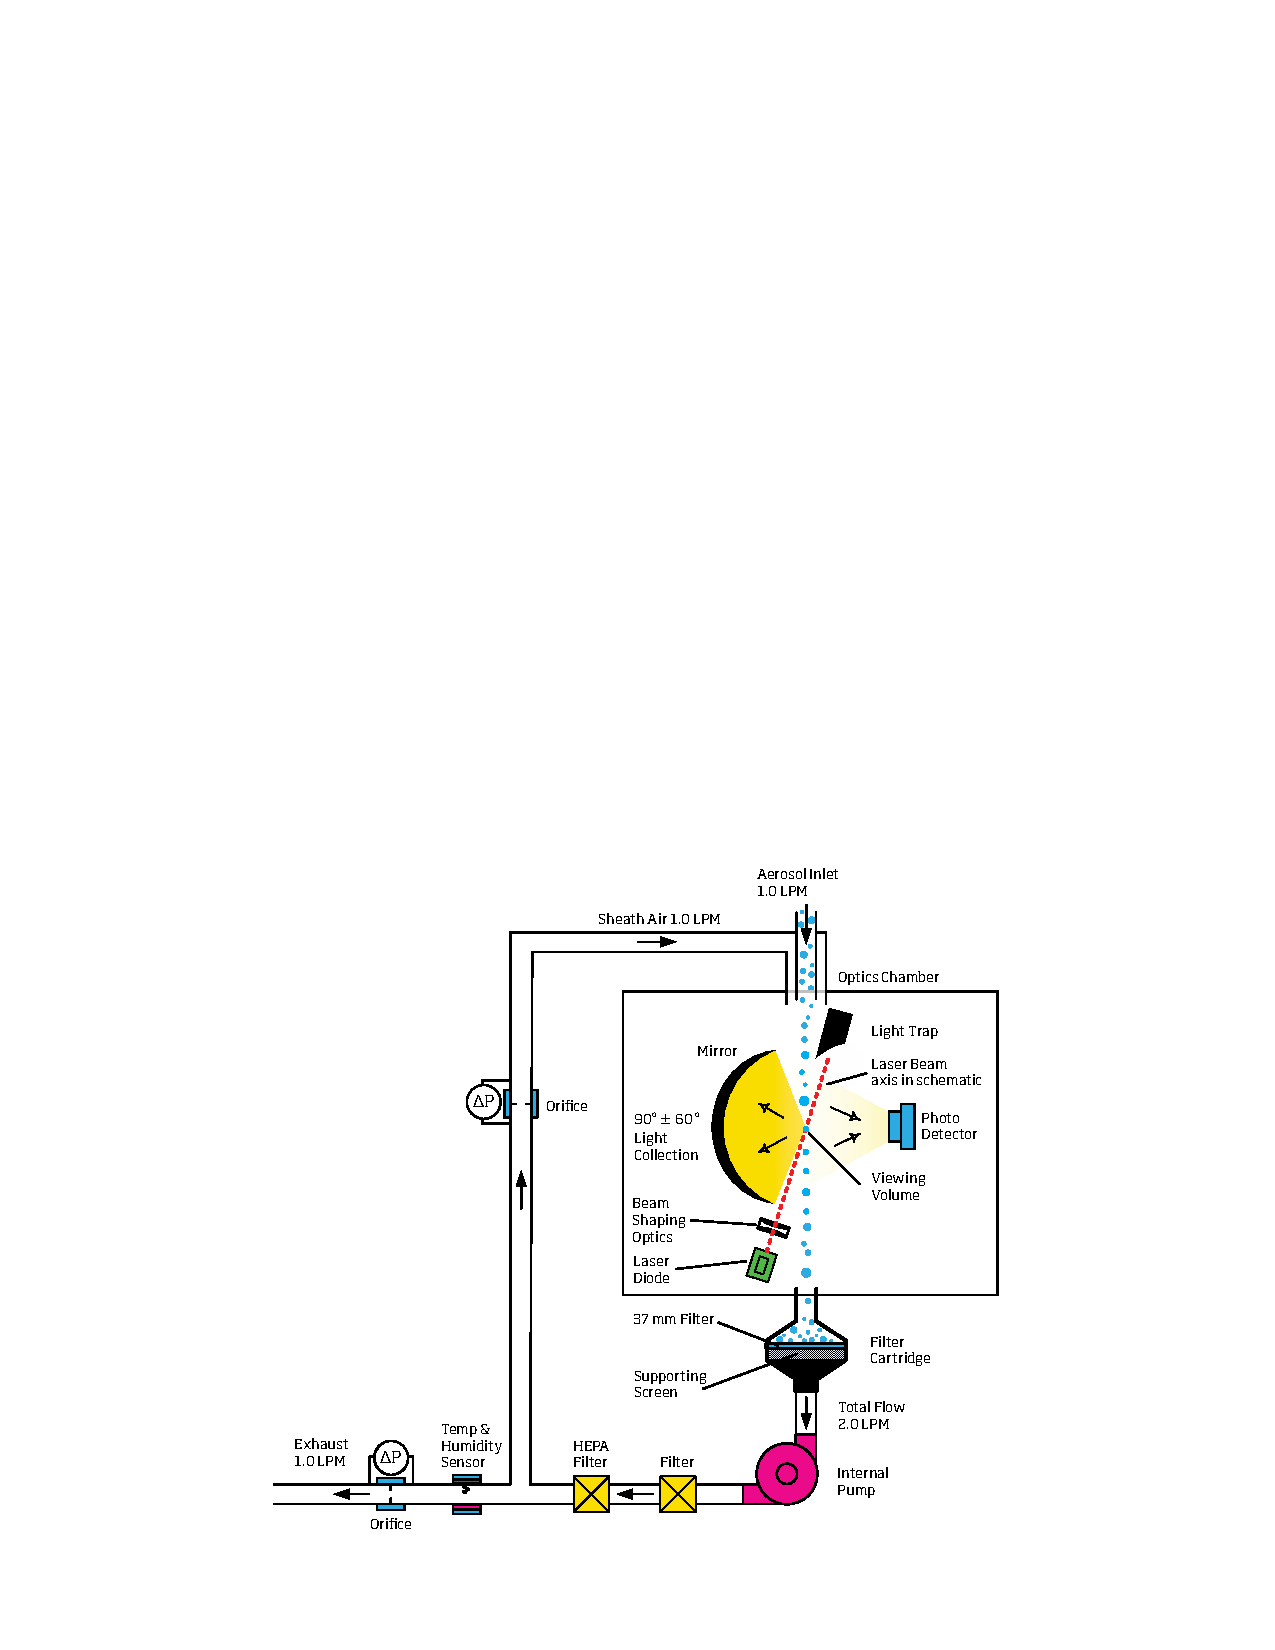
\includegraphics[width=.45\linewidth]{gfx/measuring_dev/ops_3330.pdf}}
	\caption[Messverfahren des FMPS und OPS]
	{Messverfahren des FMPS und OPS}
	\label{fig:laser_schwert}
\end{figure}

Ein wesentlicher Leistungsunterschied zwischen dem FMPS 3091 und OPS 3330 ist das Volumen des Aerosol-Tr\"{a}gergasgemisch, welches von beiden im Verh\"{a}ltnis 1:4 angesaugt wird. Der OPS arbeitet mit $5 L/min$, w\"{a}rend der FMPS mit $50 L/min$ arbeitet. Ein Teil des Luftgemisches wird dabei vom Ger\"{a}t gefiltert und dazu genutzt, den Aerosolstrom zum Messvolumen zu f\"{u}hren.